\documentclass[12pt,twoside]{article} 
\usepackage{amsmath, amssymb} 
\usepackage{graphicx}
\usepackage{amsmath} 
\usepackage[active]{srcltx} 
\usepackage{amssymb} 
\usepackage{amscd} 
\usepackage{makeidx} 
\usepackage{amsthm} 
\usepackage{algpseudocode} 
\usepackage{algorithm}
\usepackage[spanish, activeacute]{babel}
\usepackage[utf8]{inputenc}

\renewcommand{\baselinestretch}{1}
\setcounter{page}{1}
\setlength{\textheight}{21.6cm}
\setlength{\textwidth}{14cm}
\setlength{\oddsidemargin}{1cm}
\setlength{\evensidemargin}{1cm}
\pagestyle{myheadings}
\thispagestyle{empty}
\markboth{\small{Pr\'actica 5. Fernando Rivera, Alejandro Contreras}}{\small{.}}

\begin{document}
\centerline{\bf An\'alisis de Algoritmos, Sem: 2020-1, 3CV2, Pr\'actica 5}
\centerline{}
\centerline{25 - 09 - 2019}
\begin{center}
\Large{\textsc{Pr\'actica 5: Algoritmos de Ordenación}}
\end{center}
\centerline{}
\centerline{\bf {Rivera Paredes Fernando Daniel, Contreras Paredes Alejandro.}}
\centerline{}
\centerline{Escuela Superior de C\'omputo}
\centerline{Instituto Polit\'ecnico Nacional, M\'exico}
\centerline{$ferny036@hotmail.com, acontrerasparedes@hotmail.com$}
\newtheorem{Theorem}{\quad Theorem}[section] \newtheorem{Definition}[Theorem]{\quad Definition} \newtheorem{Corollary}[Theorem]{\quad Corollary} \newtheorem{Lemma}[Theorem]{\quad Lemma} \newtheorem{Example}[Theorem]{\quad Example} \bigskip
\textbf{Resumen:} Hablaremos de 3 algoritmos de ordenación diferentes a lso que hemos visto en clase, donde cada uno es diferente en si, aclarando por ejemplo, que existen algoritmos que dependen de otros, o bien que su cuerpo es lo 
suficientemente complejo para facilitar o reducir el nivel de complejidad.
\centerline{}
{\bf Palabras Clave:} CocktailSort, BucketSort, InsertSort, RadixSort, Ordenamiento
\newpage

\section{Introducción}
El ordenamiento es una labor común que realizamos continuamente. ¿Pero te has preguntado qué es ordenar? ¿No? Es que es algo tan corriente en nuestras vidas que no nos detenemos a pensar en ello. Ordenar es simplemente colocar información de 
una manera especial basándonos en un criterio de ordenamiento. En la computación el ordenamiento de datos también cumple un rol muy importante, ya sea como un fin en sí o como parte de otros procedimientos más complejos. Se han desarrollado 
muchas técnicas en este ámbito, cada una con características específicas, y con ventajas y desventajas sobre las demás. Aquí voy a mostrarte algunas de las más comunes, tratando de hacerlo de una manera sencilla y comprensible.
\centerline{}
Es por eso que en esta práctica analizaremos 3 algoritmos de ordenamiento de tal manera que podamos llegar a un conclusión sobre su uso y determinar cual se optaría por utilizar en un desempeño labral o de ejercicios para funciones explicitas
dentro de metodos o metodologías implementadas a lo alrgo del desarrollo de proyectos con el fin de ayudar a entender y brindar el mayor conocimiento de cada uno de estos algoritmos.
\newpage
\section{Conceptos B\'asicos} 
\subsection{\textbf{BucketSort}}
\setlength{\parindent}{1.5em}El ordenamiento por casilleros (bucket sort o bin sort, en inglés) es un algoritmo de ordenamiento que distribuye todos los elementos a ordenar entre un número finito de casilleros. Cada casillero sólo puede contener 
los elementos que cumplan unas determinadas condiciones. En el ejemplo esas condiciones son intervalos de números. Las condiciones deben ser excluyentes entre sí, para evitar que un elemento pueda ser clasificado en dos casilleros distintos. 
Después cada uno de esos casilleros se ordena individualmente con otro algoritmo de ordenación (que podría ser distinto según el casillero), o se aplica recursivamente este algoritmo para obtener casilleros con menos elementos. Se trata de 
una generalización del algoritmo Pigeonhole sort. Cuando los elementos a ordenar están uniformemente distribuidos la complejidad computacional de este algoritmo es de O(n).

El algoritmo contiene los siguientes pasos:
\begin{enumerate}
  \item Crear una colección de casilleros vacíos
  \item Colocar cada elemento a ordenar en un único casillero 
  \item Ordenar individualmente cada casillero
  \item Devolver los elementos de cada casillero concatenados por orden
\end{enumerate}

\subsection{\textbf{CocktailSort}}
\setlength{\parindent}{1.5em}
El ordenamiento de burbuja bidireccional (cocktail sort en inglés) es un algoritmo de ordenamiento que surge como una mejora del algoritmo ordenamiento de burbuja.

La manera de trabajar de este algoritmo es ir ordenando al mismo tiempo por los dos extremos del vector. De manera que tras la primera iteración, tanto el menor como el mayor elemento estarán en sus posiciones finales. De esta manera se reduce 
el número de comparaciones aunque la complejidad del algoritmo sigue siendo $O(n^2)$.

Hacemos un recorrido ascendente (del primer elemento al último), cogemos el primer elemento y lo comparamos con el siguiente, si el siguiente es menor lo pasamos al puesto anterior, de esta forma al final de la lista nos queda el mayor. 
Una vez terminada la serie ascendente, hacemos un recorrido descendente (del último elemento al primero) pero esta vez nos quedamos con los menores a los que vamos adelantando posiciones en vez de retrasarlas como hicimos en la serie ascendente. 
Repetimos las series alternativamente pero reduciendo el ámbito en sus extremos pues ya tendremos allí los valores más bajos y más altos de la lista, hasta que no queden elementos en la serie; en el pseudocódigo de ejemplo: Hasta (izq $>$ der).

\begin{figure}[t]
  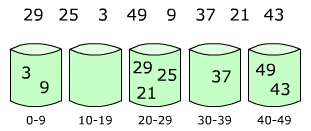
\includegraphics[height=0.25\textwidth]{Figure1}
  \centering
  \caption{BucketSort}
\end{figure}

\subsection{\textbf{RadixSort}}
\setlength{\parindent}{1.5em}Es un algoritmo de ordenamiento que ordena enteros procesando sus dígitos de forma individual. Como los enteros pueden representar cadenas de caracteres (por ejemplo, nombres o fechas) y, especialmente, números en 
punto flotante especialmente formateados, radix sort no está limitado sólo a los enteros.
Este método se puede considerar como una generalización de la clasificación por urnas.
Consiste en hacer diversos montones de fichas, cada uno caracterizado por tener en sus componentes un mismo digito (letra si es alfabética) en la misma posición; estos montones se recogen en orden ascendente y se reparte en montones según 
el siguiente digito de la clave.
\begin{figure}[t]
  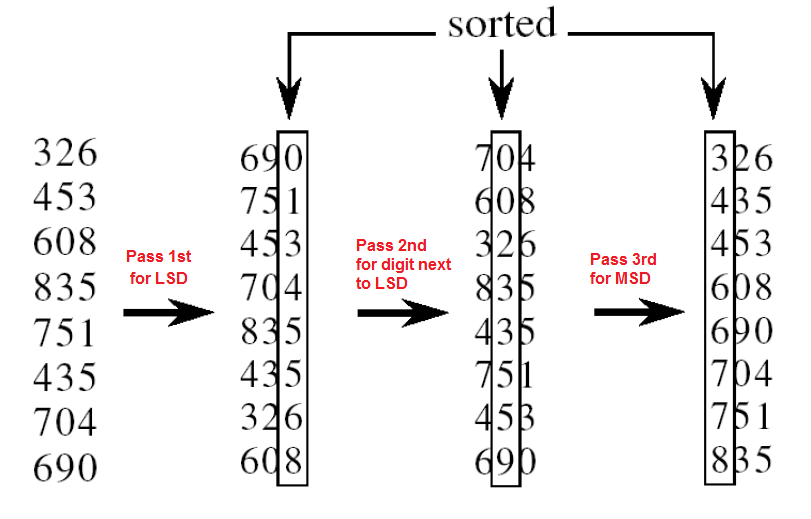
\includegraphics[height=0.5\textwidth]{Figure2}
  \centering
  \caption{RadixSort}
\end{figure}

\newpage
\section{Experimentaci\'on y Resultados}
\centerline{}
\subsection{\textbf{BucketSort}}
\begin{algorithm}
  \caption{BucketSort}\label{euclid}
  \begin{algorithmic}[1]
  \Function{BucketSort}{$A[0, ..., m-1], n$}
      \State $buckets \gets n$ list of buckets                          \Comment $O(1)$
      \For{$i = 1$ \textbf{to} tam of $A$}                              \Comment $O(n)$
        \State $c \gets$ find adecuated bucket                          \Comment $O(1)$
        \State insert $A[i]$ in $buckets[c]$                            \Comment $O(1)$
      \EndFor
      \For{$i = 1$ \textbf{to} $n$}                                     \Comment $O(n)$
        \State sort($buckets[i]$)                                       \Comment $O:$ depends of sort algorithm
      \EndFor
      \State \textbf{return} concatenate of buckets[0]...buckets[n - 1] \Comment $O(1)$
  \EndFunction
  \end{algorithmic}
\end{algorithm}

La cual para verificar analíticamente su grado de complejidad de acuerdo a los comentarios, de una manera simplificada lo podemos ver de la siguiente
manera: 

\centerline{$T(n) = O(1)+O(n)[2*O(1)]+O(n)*S+O(1)$}
\centerline{}
\centerline{donde: $S = s(n)$}
\centerline{}
\centerline{donde: $O(g(n))_{1} + O(g(n))_{2}+\cdots+O(g(n))_n = O(g(n))$}
\centerline{}
\centerline{$\Rightarrow T(n) = O(1)+O(n)[2*O(1)]+O(n)[S]$}
\centerline{}
\centerline{donde: $O(f(n)) * O(g(n))= O(f(n)*g(n))$}
\centerline{}
\centerline{$\Rightarrow T(n) = O(1) + O(n) + O(n)*S$}
\centerline{}
\centerline{donde: $O(f(n)) + O(g(n)) = O(h(n))$}
\centerline{y $h(n)$ es la funci\'on con mayor jeraqu\'ia respecto a $g(n)$ y $f(n)$}
\centerline{}
\centerline{$\therefore T(n) \in S*O(n) \| S = s(n) $}

Podemos notar que el algoritmo se comporta de manera extraña de tal manera que supone una complejidad lineal y depende totalmente
de la funcion de ordenamiento, aun si asi fuese de complejidad $O(n^2)$, o $O(1)$ la complejidad minima obtenida sería $O(n)$
\begin{figure}
  \centering
    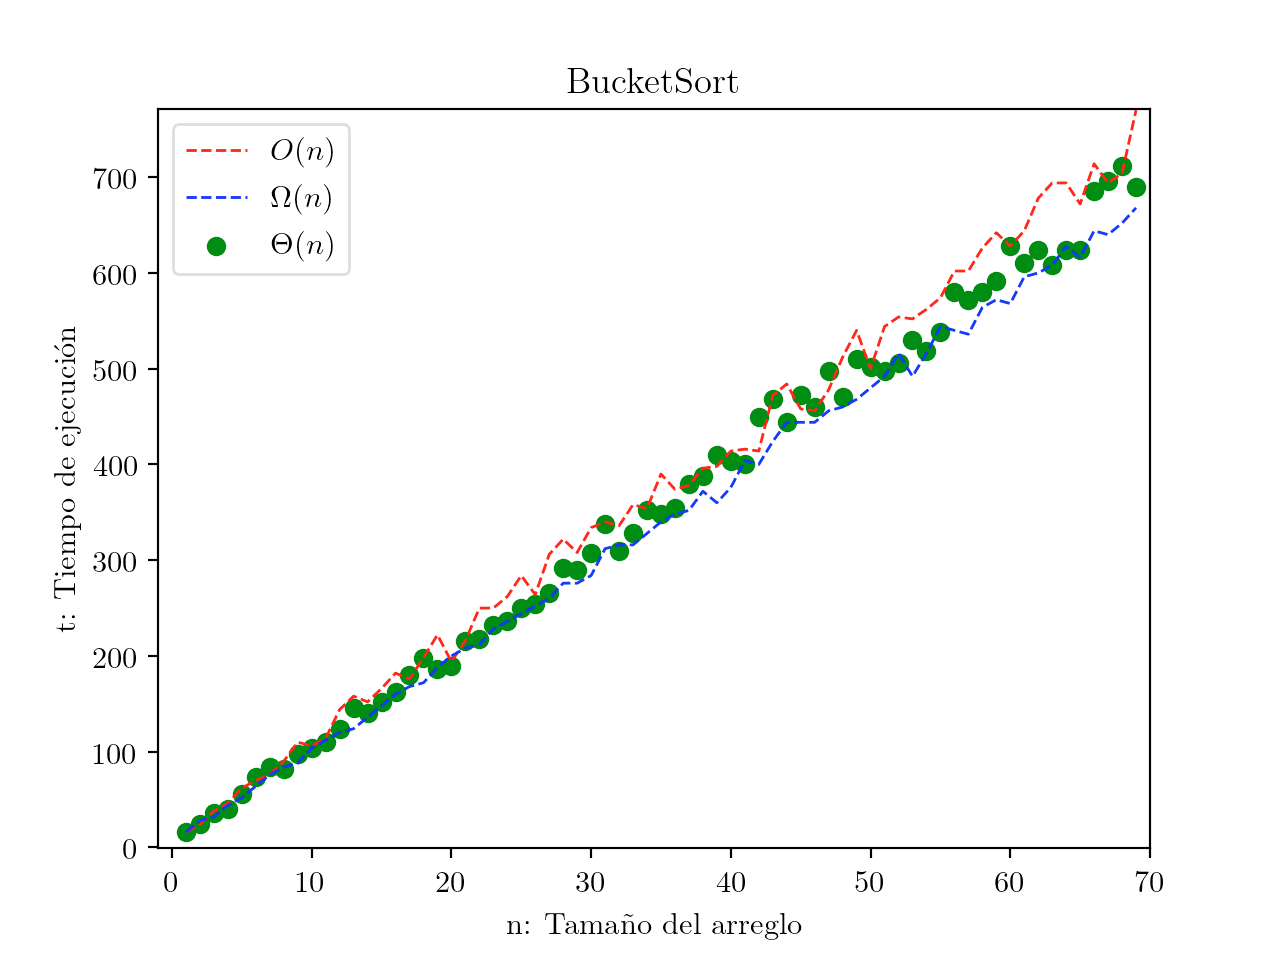
\includegraphics[height=0.75\textwidth]{Figure3}
  \caption{Comportamiento del algoritmo BucketSort}
  \label{fig:ejemplo1}
\end{figure}

\subsection{\textbf{CocktailSort}}
\begin{algorithm}
  \caption{CocktailSort}\label{euclid}
  \begin{algorithmic}[1]
  \Function{CocktailSort}{$A[0, ..., n-1]$}
    \State $n \gets tam(A)$                     \Comment $O(1)$
    \State $comb \gets true$                    \Comment $O(1)$
    \State $init \gets 0$                       \Comment $O(1)$
    \State $final \gets n - 1$                  \Comment $O(1)$
    \While $comb = true$                        \Comment $O(n)$
      \State $comb \gets false$                 \Comment $O(1)$
      \For{$i = inicio$ \textbf{to} $final$}    \Comment $O(n)$
        \If {$A[i] > A[i + 1]$}                 \Comment $O(1)$
          \State $change(A[i], A[i + 1])$       \Comment $O(1)$
          \State $comb = true$                  \Comment $O(1)$
        \EndIf
      \EndFor
      \If{$comb = false$}                       \Comment $O(1)$
        \State $break$                          \Comment $O(1)$
      \EndIf
      \State $comb = false$                     \Comment $O(1)$
      \State $final = final - 1$                \Comment $O(1)$
      \For{$i = final$ \textbf{to} $inicio$}    \Comment $O(n)$
        \If {$A[i] > A[i + 1]$}                 \Comment $O(1)$
          \State $change(A[i], A[i + 1])$       \Comment $O(1)$
          \State $comb = true$                  \Comment $O(1)$
        \EndIf
      \EndFor
      \State $inicio = inicio + 1$              \Comment $O(1)$
    \EndWhile
    \State \textbf{return} $A$ \Comment $O(1)$  \Comment $O(1)$
  \EndFunction
  \end{algorithmic}
\end{algorithm}
El algoritmo de \textbf{CocktailSort} podemos analizarlo de forma que:

\centerline{$T(n) = 4*O(1)+O(n)[O(n)[3*O(1)]+ 3*O(1)+2*O(1)+O(n)[3*O(1)]] + 2*O(1)$}
\centerline{}
\centerline{donde: $O(g(n))_{1} + O(g(n))_{2}+\cdots+O(g(n))_n = O(g(n))$}
\centerline{}
\centerline{$\Rightarrow T(n) = O(1)+O(n)[O(1) + O(n)[O(1)]]$}
\centerline{}
\centerline{$\Rightarrow T(n) = O(1) + O(n)*O(n)$}
\centerline{}
\centerline{donde: $O(f(n)) * O(g(n))= O(f(n)*g(n))$}
\centerline{}
\centerline{donde: $O(f(n)) + O(g(n)) = O(h(n))$}
\centerline{y $h(n)$ es la funci\'on con mayor jeraqu\'ia respecto a $g(n)$ y $f(n)$}
\centerline{}
\centerline{$\therefore T(n) \in O(n^2)$}

Analizando el algoritmo podemos concluir que es un de los peores algoritmos de ordenamiento que se pueden implementar, sobretodo, suele ser
complejo el intentar interpretarlo, su complejidad solo esta por debajo del \textbf{PogoSort} y del \textbf{BubbleSort}, sin embargo se
podria ayudar a mejorar su complejidad de alguna otra manera como técnicas de divide y venceras o simplemente implementando con cómputo paralelo.

\begin{figure}
  \centering
    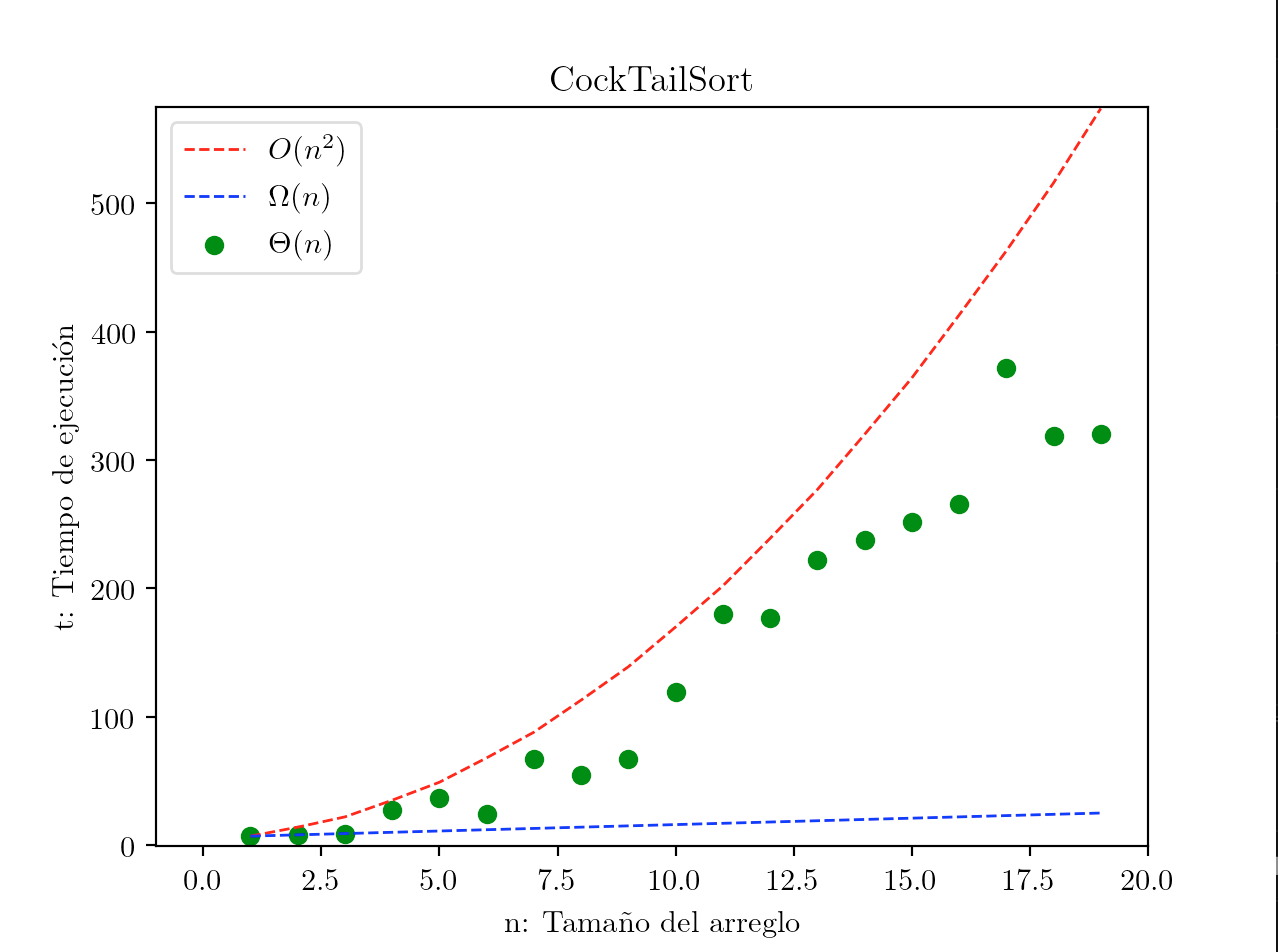
\includegraphics[height=0.75\textwidth]{Figure4}
  \caption{Comportamiento de CocktailSort}
  \label{fig:ejemplo3}
\end{figure}
\subsection{\textbf{RadixSort}}
\begin{algorithm}
  \caption{RadixSort}\label{euclid}
  \begin{algorithmic}[1]
  \Function{RadixSort}{$A[0, ..., n-1]$}
    \State $n \gets tam(A)$                                                 \Comment $O(1)$
    \State $digitPosition \gets 1$                                          \Comment $O(1)$
    \State $result[n]$                                                      \Comment $O(1)$
    \For{$j = 1$ \textbf{to} $d$}                                           \Comment $O(d)$
      \State $count[10]$                                                    \Comment $O(1)$
      \For {$i = 0$ \textbf{to} $n$}                                        \Comment $O(n)$
        \State $count[(A[i]/digitPosition) \% 10]++$                        \Comment $O(1)$
      \EndFor                                 
      \For {$i = 0$ \textbf{to} $n$}                                        \Comment $O(n)$        
        \State $count[(A[i]/digitPosition) \% 10]++$                        \Comment $O(1)$
      \EndFor
      \For {$i = n-1$ \textbf{to} $0$}                                      \Comment $O(n)$
        \State $result[count[(A[i]/digitPosition) \% 10] - 1] \gets A[i]$   \Comment $O(1)$
        \State $count[(A[i]/digitPosition) \% 10]--$                        \Comment $O(1)$
      \EndFor
      \For {$i = 0$ \textbf{to} $n$}                                        \Comment $O(n)$
        \State $A[i] \gets result[i]$                                       \Comment $O(1)$
      \EndFor

      \State $digitPosition \gets digitPosition*10$                         \Comment $O(1)$
    \EndFor
    \State \textbf{return} concatenate of buckets[0]...buckets[n - 1]       \Comment $O(1)$
  \EndFunction
  \end{algorithmic}
\end{algorithm}

El algoritmo de \textbf{RadixSort} podemos analizarlo de forma que:

\centerline{$T(n) = 3*O(1)+O(d)[O(1) + O(n)[O(1)]+ O(n)[O(1)] + O(n)[2*O(1)] + 2*O(1)]$}
\centerline{}
\centerline{donde: $d = $ cantidad de digitos o letras de la entrada}
\centerline{}
\centerline{donde: $O(g(n))_{1} + O(g(n))_{2}+\cdots+O(g(n))_n = O(g(n))$}
\centerline{}
\centerline{$\Rightarrow T(n) = O(1)+O(d)[O(1) + O(n)[O(1)]]$}
\centerline{}
\centerline{$\Rightarrow T(n) = O(1) + O(d)*O(n)$}
\centerline{}
\centerline{donde: $O(f(n)) * O(g(n))= O(f(n)*g(n))$}
\centerline{}
\centerline{$\Rightarrow T(n) = O(1) + O(dn)$}
\centerline{}
\centerline{donde: $O(f(n)) + O(g(n)) = O(h(n))$}
\centerline{y $h(n)$ es la funci\'on con mayor jeraqu\'ia respecto a $g(n)$ y $f(n)$}
\centerline{}
\centerline{$\therefore T(n) \in O(dn)$}

De acuerdo al algortimo podemos concluir que puede tener un orden lineal de acuerdo a la cantidad de digitos, sin embargo odria pasar algo curioso
respecto a la cantidad de digitos, y es que si siempre hay la misma cantidad de digitos como elementos de los arreglos, esto quiere decir que el factor
de complejidad incrementa a $O(n^2)$, aunque en la realidad esto es casi imposible debido a que se puede tener una base de datos con trillones de datos
pero hay pocas expresiones matematicas, como $\pi$ o $e$, que pueden tener esa cantidad de cifras simplemente por el hecho de ser irracionales.

\begin{figure}
  \centering
    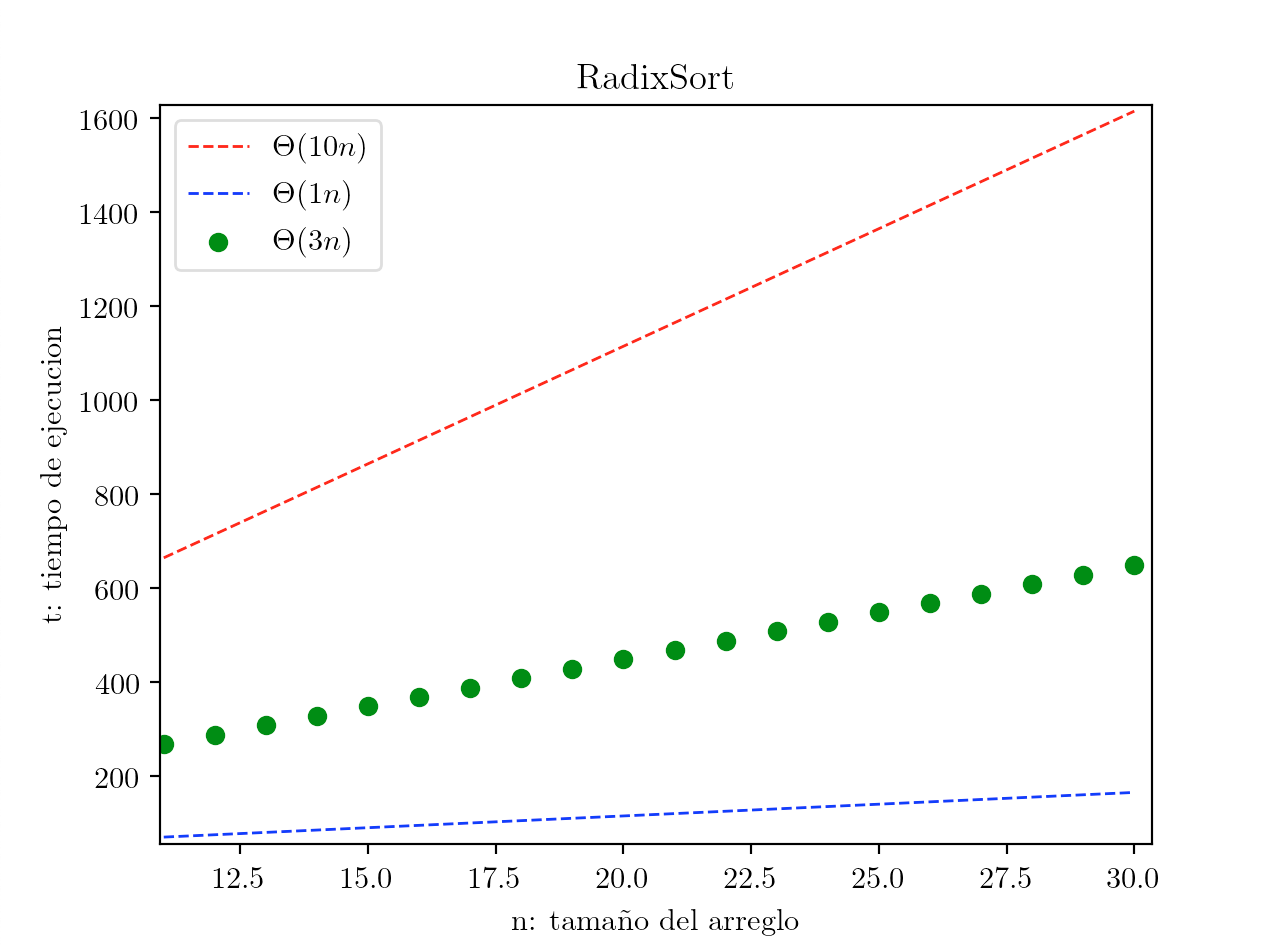
\includegraphics[height=0.75\textwidth]{Figure5}
  \caption{Comportamiento de RadixSort}
  \label{fig:ejemplo3}
\end{figure}

\begin{figure}[!h]
	\centering
	\begin{minipage}[t]{10cm}
		\centering
		
\includegraphics[scale=0.2]{Foto1}
		\caption{Alejandro Contreras Paredes}
	\end{minipage}
	\hspace{18cm}
	\begin{minipage}[t]{10cm}
		\centering
		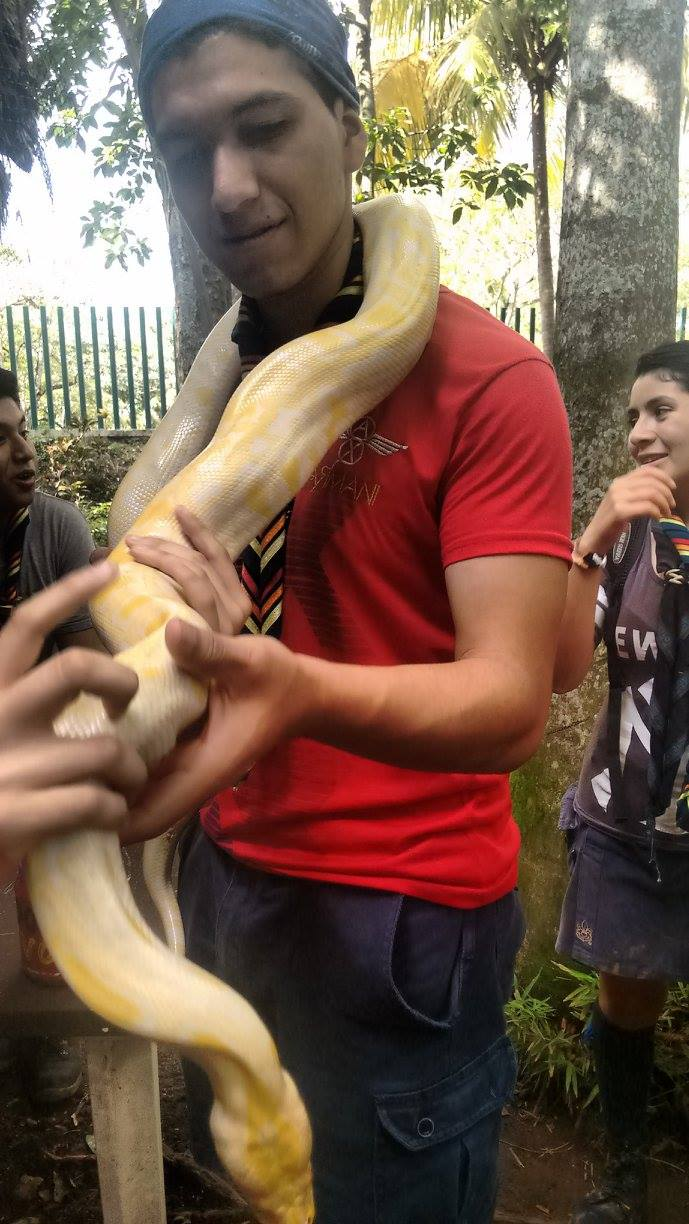
\includegraphics[scale=0.2]{Foto2}
		\caption{Rivera Paredes Fernando Daniel}
	\end{minipage}
\end{figure}
\newpage
\section{Conclusiones}
\textbf{Conclusion Alejandro Contreras Paredes}\\
Para el desarrollo de esta practica usamos los algoritmos que fueron desarollados en clase, de los cuales, uno estaba incompleto
lo que represento un problema a la hora de la codificación, esto represento un pequeño retraso pero finalmente pudimos solucionarlo. Por otra
parte, esta practica reafirma la teoria de la complejidad de los algoritmos recursivos y finalmente las graficas fueron realizadas conforme a las indicaciones
especificadas.\\\\
\textbf{Conclusion Fernando Daniel Rivera Paredes}\\

Al desarrollo de esta práctica fue escencial determinar cual algoritmo implementariamos y el porque, cuando optamos por elegir 3 de tantos y las variantes que
estos conllevaban fue algo complejo, sin embargo manejamos un interés sobre 3 puntos ideas, \textit{retomar algún algoritmo viejo, un algoritmo actual, y un 
algoritmo óptimo o con una carácteristica distinta} a la que generalmente trabajabamos, tal como el caballito de batalla de \textbf{BubbleSort} pero mejorado,
hablando en si de \textbf{CocktailSort}; el algoritmo \textbf{BucketSort} con la caracteristica que requiere de otro algoritmo de ordenamiento para poder funcionar
correctamente, creando tal dependencia entre sí; por último elegimos \textbf{RadixSort} como  un enfoque moderno en su forma mas natural, ya que este tiene variaciones
que lo hacen funcionar de distintas maneras. Un punto muy importante es que de acuerdo a la manera teórica, no sabemos el porque del algoritmo \textbf{BucketSort}
a pesar de que internamente utilicemos \textbf{InsertSort} para ordenar los elementos, no se logran graficar de una manera explicita, redujendo su complejidad a $O(n)$.


\section{Bibliograf\'ia}

\begin{thebibliography}{9}
  \bibitem{book} 
  Cormen, T. and Leiserson, C.
  \textit{Introduction to algorithms.} 
  3rd edition.Cambridge, Massachusetts: Massachusetts Institute of Technology, 2009.

  \bibitem{ie} 
  Moyano, N.
  \textit{Análisis de algoritmos}.
  Medium. Available at: $www.lcc.uma.es/~av/Libro/CAP3.pdf$'[Accessed 03 Sep. 2019].
\end{thebibliography}
\end{document}
